\chapter{Theoretische Grundlagen}
Der Bicycle Computer basiert auf Energy Harvesting. Was Energie ernten bedeutet und welche Art von Energy Harvesting in dieser Arbeit angewandt wird, wird im ersten Unterkapitel \ref{t_harvesting} beschrieben. Im folgenden Unterkapitel \ref{t_energy_management} geht es um Ansätze zum Sammeln und Weiterleiten von Energie. Da die in Unterkapitel \ref{t_harvesting} gewonnene Energie im $\mu$W-Bereich liegt, ist zuerst ein Sammeln der Energie notwendig, sodass Leistungen im mW-Bereich zur Verfügung stehen. Das nächste Unterkapitel \ref{t_power_management} befasst sich mit dem notwendigen Power Management. Denn die
Energie soll nicht sofort verbraucht werden. Power Management regelt, wie schnell und wie viel Energie aufs Mal verbraucht werden soll. Als letzte Stufe in der Umsetzung ist eine energiearme Kommunikation notwendig. Da bietet die Bluetooth Low Energie Technologie ideale Voraussetzungen. Das Protokoll und die Technologie werden im letzten Grundlagenteil \ref{t_ble} vorgestellt.


% 2.1-------------------------------------------------------------------
\section{Energy Harvesting}\label{t_harvesting} 

\glqq Mit Energy Harvesting ... wird die Gewinnung von elektrischer Energie in kleinen Mengen aus dem Umfeld elektronischer Geräte für deren Betrieb bezeichnet.\grqq \todo{Abstand zu klein} \cite{harvesting}. Als erstes werden Methoden zur Energiegewinnung vorgestellt (\ref{harv_arten}) und danach die im Bicycle Computer verwendete Harvesting Art genauer beschrieben (\ref{harv_bewegung}). Als letztes wird der Unterschied zwischen den Harvestingmethoden festgehalten. Denn diese Unterschiede werden in der Implementation des Bicycle Computers wichtig.


\subsection{Energy Harvesting Methoden}\label{harv_arten} 

Bekannte Methoden sind die Solarzelle, die aus der Energie der Sonnenstrahlen Strom erzeugt, die Thermogeneratoren (TEG), die aus Umgebungswärme Energie gewinnen,  passive RFID-Tags, die aus der elektromagnetischen Strahlung Energie gewinnen und der piezoelektrische Effekt, der mechanischen Druck in elektrische Spannung umwandelt. Da der im Prototyp verwendete Energy Mangement-Chip \cite{datasheet_EM85} für die Energieoptimierung von Solarzellen oder von Thermogenaratoren spezialisiert ist, werden diese zwei Methoden vorgestellt. 

\subsubsection{Energy Harvesting mit einer Solarzelle}\label{harv_solarzelle} 

Bei der Umwandlung von Elektromagnetischen Wellen (Licht) in Strom wird eine spezielle Eigenschaft des Siliziums genutzt: Führt man Silizium Energie zu, entstehen freie Ladungsträger, bzw. Elektronen und Löcher. Um aus diesen Ladungen einen elektrischen Strom zu erzeugen, ist es nötig, die erzeugten freien Ladungsträger in unterschiedliche Richtungen zu lenken; dies geschieht durch ein internes elektrisches Feld, welches durch einen p-n-Übergang erzeugt werden kann. Auf der einen Seite sammelt sich positive, auf der anderen Seite negative Ladung an. Werden diese verbunden, entsteht ein Strom (\cite{Internet_Solarzelle2}). 
Diese Harvestermethode produziert ein Gleichstrom. Grössen- und materialabhängig kann Energie im kW-Bereich gesammelt werden.

\subsubsection{Energy Harvesting mit einem TEG}\label{harv_TEG} 
TEG steht für Thermoelectric Generator und bezeichnet eine Konstruktion, die aus einem Temperaturunterschied elektrische Spannung erzeugt. Erzeugt wird die Spannung am Ende zweier metallischer Leiter aus unterschiedlichem Material, die an einem Ende verbunden sind ( \cite{Journal_TEG}). Diese Harvestermethode produziert eine Gleichspannung. Die produzierte Spannung ist vergleichsweise klein und bewegt sich im Bereich einiger 10 $\mu$V pro $1^\circ$C Temperaturdifferenz.


\subsection{Energy Harvesting über Bewegungsinduktion}\label{harv_bewegung} 
Beim Bicycle Computer wird Energie über Bewegungsinduktion gewonnen. Die Funktionsweise ist in der Machbarkeitsstudie beschrieben \cite{PA_bicycle} S.8.:

Befindet sich eine Spule in einem \textit{dynamischen} \glqq Magnetfeld\grqq, wird in der Spule eine Spannung induziert. Dies sieht man in der Formel (\ref{Formel_induzSpannung}).

\begin{equation}
    U_{ind}=-\frac{d}{dt}\intop A\,dB \ \label{Formel_induzSpannung} 
\end{equation}

Der magnetische Fluss $B$ durch die Fläche einer Spule $A$ ist gleich dem magnetischen Fluss $\phi$. Hat die Spule mehrere Wicklungen $N$, so verstärkt sich der magnetische Fluss proportional. 

 
\begin{equation}
    \frac{d}{dt} \int A\,dB=\phi\cdot N\
\end{equation}

Verläuft der magnetische Fluss $\phi$ senkrecht zur Fläche der Spule $A$ kann das Integral durch eine Multiplikation ersetzt werden (siehe Formel\ref{Formelsenkrecht}). 
 
\begin{equation}
    \frac{d}{dt} \int A\,\perp\, dB=\frac{d}{dt}\int \phi\cdot N=B\cdot A\cdot N\ \label{Formelsenkrecht} 
\end{equation} 
  
 
In diesem Fall berechnet sich die induzierte Spannung in einer Spule vereinfacht mit
\begin{equation}
    U_{ind}= - N \cdot A \cdot B
\end{equation}

Das dynamische Magnetfeld wird durch das Bewegen, oder im Fall eines Fahrrads einem Vorbeiziehen, eines Magneten an einer fix verankerten Spule erzeugt.
Die produzierte Spannung hängt von folgenden vier Faktoren ab:
\begin{enumerate}
    \item die eingeschlossene Fläche $A$ der Spule    
    \item die magnetische Flussdichte des Magneten $B$ 
    \item die Anzahl Windungen $N$ der Spule und
    \item die Bewegungsgeschwindigkeit $v$ des Magneten, welche Einfluss auf $dt$ hat
\end{enumerate}

Diese Harvestergmethode produziert einen Wechselstrom. Ein Gleichrichter und einen Kondensator zur Glättung der Rippelspannung ist nach der Energiegewinnung notwendig. Die Leistung der produzierten Spannung geht vom $\mu$W-Bereich bis zu für die Industrie optimierten Anlagen mit Leistung MW-Bereich wie z. B. durch Drehstrom-Generatoren.



\subsection{Unterschiede Harvestermethoden}\label{harv_diff} 

Unterschiede bestehen in der Art, in der die Energie zur Verfügung steht. Die nachfolgenden zwei Unterpunkte zeigen, dass zwei Differenzen auf: Punkt a verweist auf die unterschiedliche Art, in der die Energie erhältlich ist: entspricht dies einer gleichmässigen Energie, analog zum DC, oder liefert die Quelle Energie in Form von Wechselstrom? Folgt der Strom konstant oder in Pulsen? Die aufwendige Art der Energieerntung wird für den Prototypen relevant.  Der zweite Unterschied unter den Harvestermethoden ist die Leistungskurve. An welcher Stelle zwischen Kurzschluss und liegt das Leistungsmaximum? Die unterschiedlichen Leistungsmaxima der einzelnen Harvestermethoden werden unter Punkt b zusammengefasst. Beide Unterschiede werden für die Entwicklung des Prototypen über Bewegungsinduktion relevant.

\subsubsection{Gleichmässige Energie versus gepulster Energie}

\todo{Messprotokolle}
Die Solarzelle und ein TEG liefern Gleichstrom bzw. -spannung (siehe Abbildung \ref{dc}). Dadurch ist keine Gleichrichterschaltung und Glättung notwendig sind. Die durch Bewegungsinduktion gewonnene Energie ist eine Wechselspannung (siehe Abbildung \ref{ac}, aus Messprotokoll xxxx). Im Fall des Bicycle Computers ist diese gleichzeitig gepulst. Die Energie ist somit nicht konstant da, sondern nur in Zeitintervallen. Dadurch ergeben sich zwei Probleme bei der Energiegewinnung: Durch den Gleichrichter geht Energie verloren und durch die Pulsform entsteht, trotz Signalglättung über einen Kondensator, eine Rippelspannung (siehe Abbildung \ref{rippel}, aus Messsprotokoll xxxx). 

\begin{figure}[ht]
 \begin{minipage}{0.5\textwidth}
 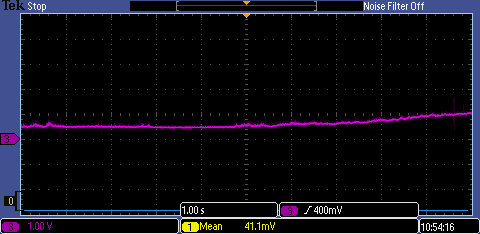
\includegraphics[width=0.9\textwidth]{2TheoretischeGrundlagen/imag/Solarstrom.PNG}
    \caption{Gleichspannung am Ausgang eines TEG}
    \label{dc} 
 \end{minipage}
 \begin{minipage}{0.5\textwidth}
     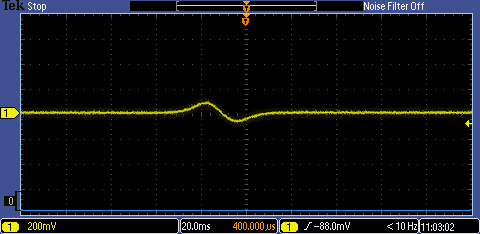
\includegraphics[width=0.9\textwidth]{2TheoretischeGrundlagen/imag/acPremospule.PNG}
    \caption{Wechselspannung als Energieform der Bewegungsinduktion}
    \label{ac} 
 \end{minipage}
\end{figure}

\begin{figure}[ht]
     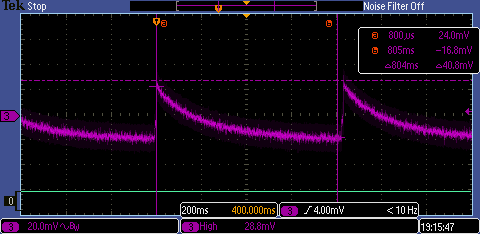
\includegraphics[width=0.45\textwidth]{2TheoretischeGrundlagen/imag/Rippel.PNG}
    \caption{Rippelspannung aufgrund der gepulsten Eingangsenergie}
    \label{rippel} 
\end{figure}



\subsubsection{Konstanter Maximum Power Point (MPP)zu dynamischem MPP}
\label{mpp_theorie_diff}

Die drei Harvester unterscheiden sich in ihrer Leistungskurve. Das Leistungsmaximum, der Maximum Power Point (MPP), liegt auf der Skala von Kurzschluss bis Leerlauf proportional an unterschiedlichen Stellen.  Bei einem TEG liegt das MPP in der Mitte dieser Skala. Die MPPT-Ratio beträgt 50\thinspace\%. Bei der Solarzelle liegt das Leistungsmaximum auf der Skala bei ca. 80\thinspace\% der maximalen Spannung. Die MPP-Ratio ist 80\thinspace\%.  Bei der Bewegungsinduktion existiert kein fixe MPP-Ratio. Wie bei der Spule, wandert das Leistungsmaximum aufgrund mehrerer Indikatoren (wie Geschwindigkeit des Magneten durch die Spule, Abstand von Magnet und Spule) auf der Skala hin und her.

Zur Verdeutlichung der Unterschiede sind für jedes Leistungsverhalten eine Abbildung angefügt. Das TEG hat unabhängig von der gewonnenen Energie und der Temperatur das Leistungsmaximum immer bei 50\thinspace\%. Die Abbildung \ref{teg} zeigt, dieses unabhängige Verhalten. 

\begin{figure}[ht]
 \begin{minipage}[t]{0.5\textwidth}
 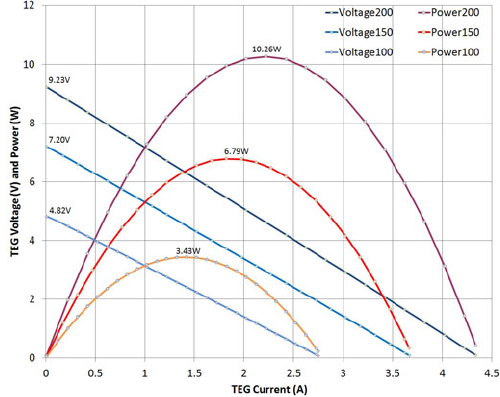
\includegraphics[width=0.9\textwidth]{2TheoretischeGrundlagen/imag/MPPTEG.png}
\caption{MPP TEG (\cite{MPP_TEG})}
\label{teg} 
 \end{minipage}
 \begin{minipage}[t]{0.5\textwidth}
    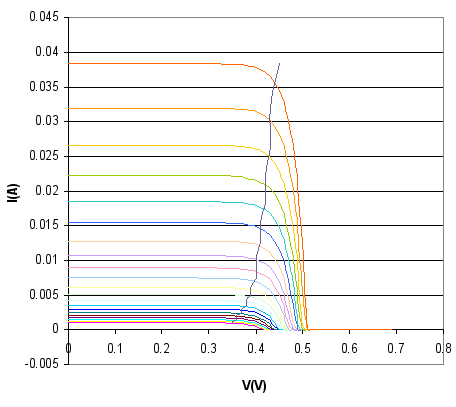
\includegraphics[width=0.9\textwidth]{2TheoretischeGrundlagen/imag/MPPSolar.png} 
    \caption{MPP Solarzelle (\cite{mpp_solar})}
    \label{mppsolar}
 \end{minipage}
\end{figure}

Abbildung \ref{mppsolar} zeigt, dass das Leistungsmaximum bei der Solarzelle unabhängig von der zur Verfügung stehenden Energie immer bei 80\thinspace\% liegt.

Die Stelle des Leistungsmaximums wandert bei einer Spule und somit bei der Bewegungsinduktion auf der Skala. Exemplarisch sind drei MPPT-Ratios einer Spule in der Abbildung \ref{bildspule} abgebildet. In dieser Abbildung zeigt sich der Einfluss des Abstands der Spule vom Magnetfeld auf die Stelle der maximalen Leistung. Diese Abbildung wurde ausgewählt, weil beim Ausmessen des Harvesters der Abstand des Magneten als einer der Einflüsse festgestellt wurde. Im Kapitel \ref{ch_resultat} Resultat sind die ausgemessenen Leistungskurven des Prototypen in der Graphik \ref{mpp_resultat_harvester} abgebildet. Die Leistungskurven wurden für verschiedene Geschwindigkeiten aufgenommen und es zeit sich, dass bei der Harvesterschaltung analog zur Spule, die MPPT-Ratio wandert. Für den theoretischen Teil wurde die MPPT-Kurven des Harverster starkt geglättet und vereinfacht(siehe untenstehende Abbildung \ref{bild_harvester}). So ist der Effekt der Verschiebung des Leistungsmaximums besser ersichtlich wird. Es lässt sich grob über die MPPT-Ratio des Bicycle Computers sagen, dass sie sich zwischen 35 - 75\thinspace\% bewegt.

\begin{figure}[ht]
 \begin{minipage}[t]{0.5\textwidth}
   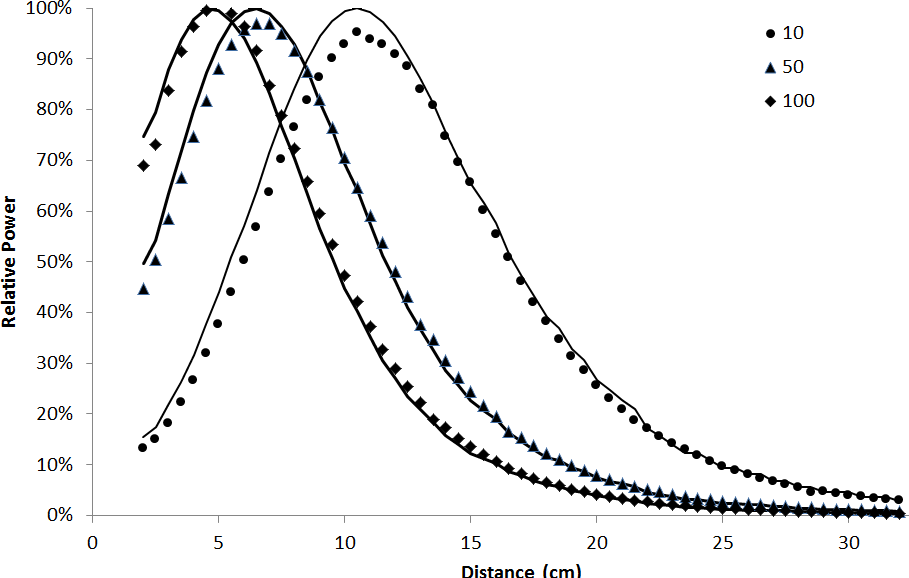
\includegraphics[width=0.9\textwidth]{2TheoretischeGrundlagen/imag/MPPSpule.png}
   \caption{MPP Spule (\cite{MPP_Spule})}
   \label{bildspule} 
 \end{minipage}
 \begin{minipage}[t]{0.5\textwidth}
   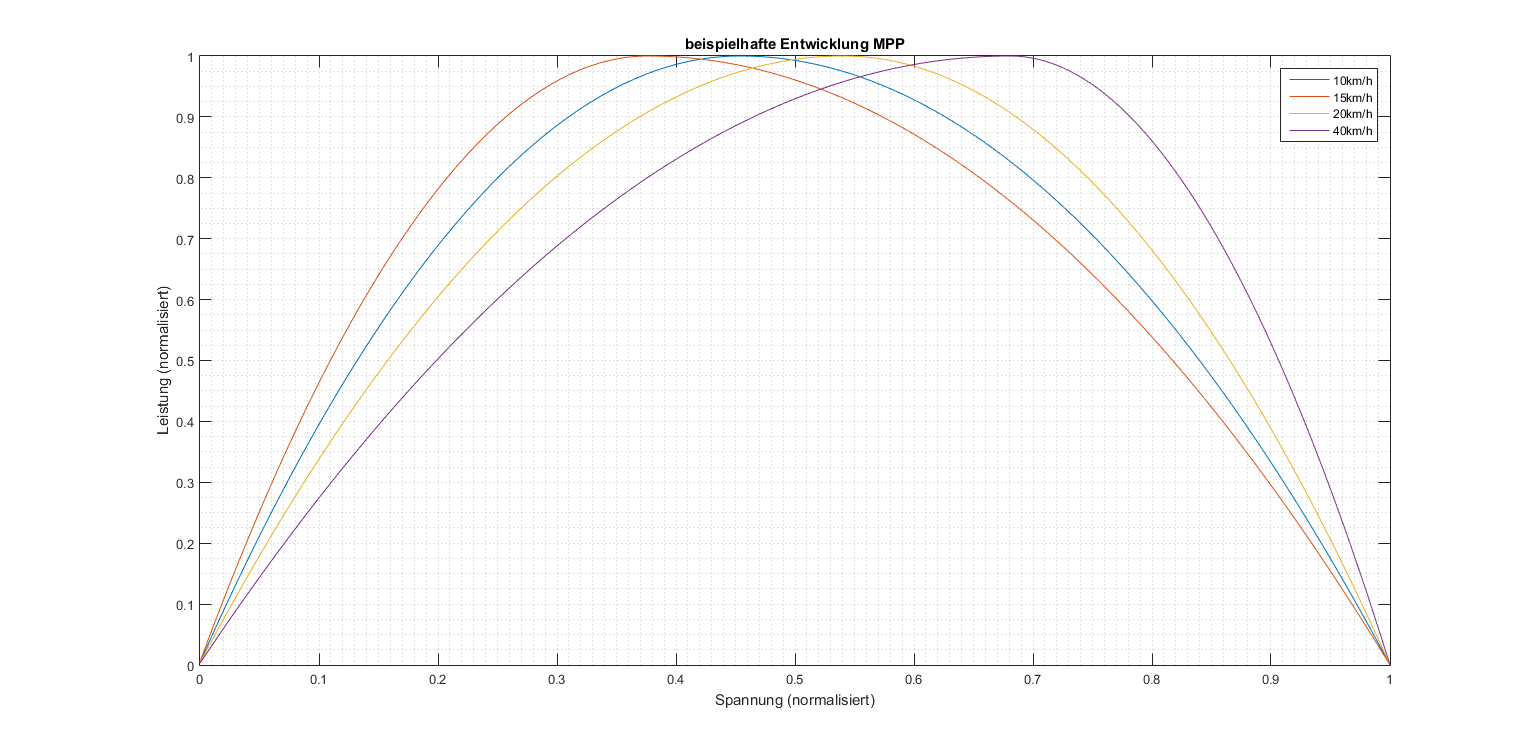
\includegraphics[width=0.9\textwidth]{2TheoretischeGrundlagen/imag/MPPharvesterTheorie.png}
   \caption{MPP Harvester (\cite{MPP_Harv})}
   \label{bild_harvester} 
 \end{minipage}
\end{figure}

% 2.2-------------------------------------------------------------------
\section{Energy Management}\label{t_energy_management} 

Der Harvester des Bicycle Computer erntet eine gepulste Energie im $\mu$J-Bereich. Um diese für eine Applikation zu verwenden, müssen die geringen Energieportionen summiert werden. Sind Energiemengen im höheren $\mu$J-Bereich verfügbar, kann die Energie kontrolliert freigegeben werden. 

Energy Management bezeichnet das der Energie in Speichern, das Regeln des Inputs, damit die maximale Leistung aus der Quelle bezogen werden kann, das Aufwärtswandeln von Spannung oder Strom auf den geforderten Wert und die kontrollierte Freigabe.

In der Bachelorarbeit ist das Verwenden des Chip EM8500 vorgegeben. Der EM8500 ist ein Power Management Controller für den Low Power-Bereich. Das Datenblatt des EM8500 ist der CD beigelegt.  Als erstes wird das kontrollierte Energiespeichern anhand dieses Chips erklärt. Danach folgt die Umsetzung des Maximum Power Point Trackings (MPPT) und eine kurze Erklärung der Wirkung des Boosters auf das Energy Managments. Zuletzt wird auf das freischalten von Ausgängen eingegangen, da dies für das Verwenden der Energie die wesentliche Schnittstelle ist. 

\subsection{Kontrollierte Energiespeicherung}
\label{speicher_konzept}

Bei einer Low Power Harvesting Applikation ist wesentlich, dass vor der Verwendung der Energie durch einen Microkontroller, genug Energie in Speichern gesammelt wurde. Dies ist in der Abbildung \ref{em_grundprinzip} dargestellt. Sie zeigt, dass für die Freigabe der Energie an eine Applikation, das Signal der Speisung der Applikation wird als VSUP bezeichnet, erst nach dem Erreichen eines gewissen Speicherzustands erfolgt. Die Höhe des Speicherwertes kann im Register v\_bat\_min\_low eingetragen werden. Die Ladespannung des sogenannten Primärspeichers, dem Short Time Storage (STS), ist mit VSTS in der Abbildung \ref{em_grundprinzip} abgebildet.

\todo{Graphik falsch: VSUP auf batminlow. vsts geht auf v bat min hi dis}
\begin{figure}[ht]
 \begin{minipage}[t]{0.5\textwidth}
   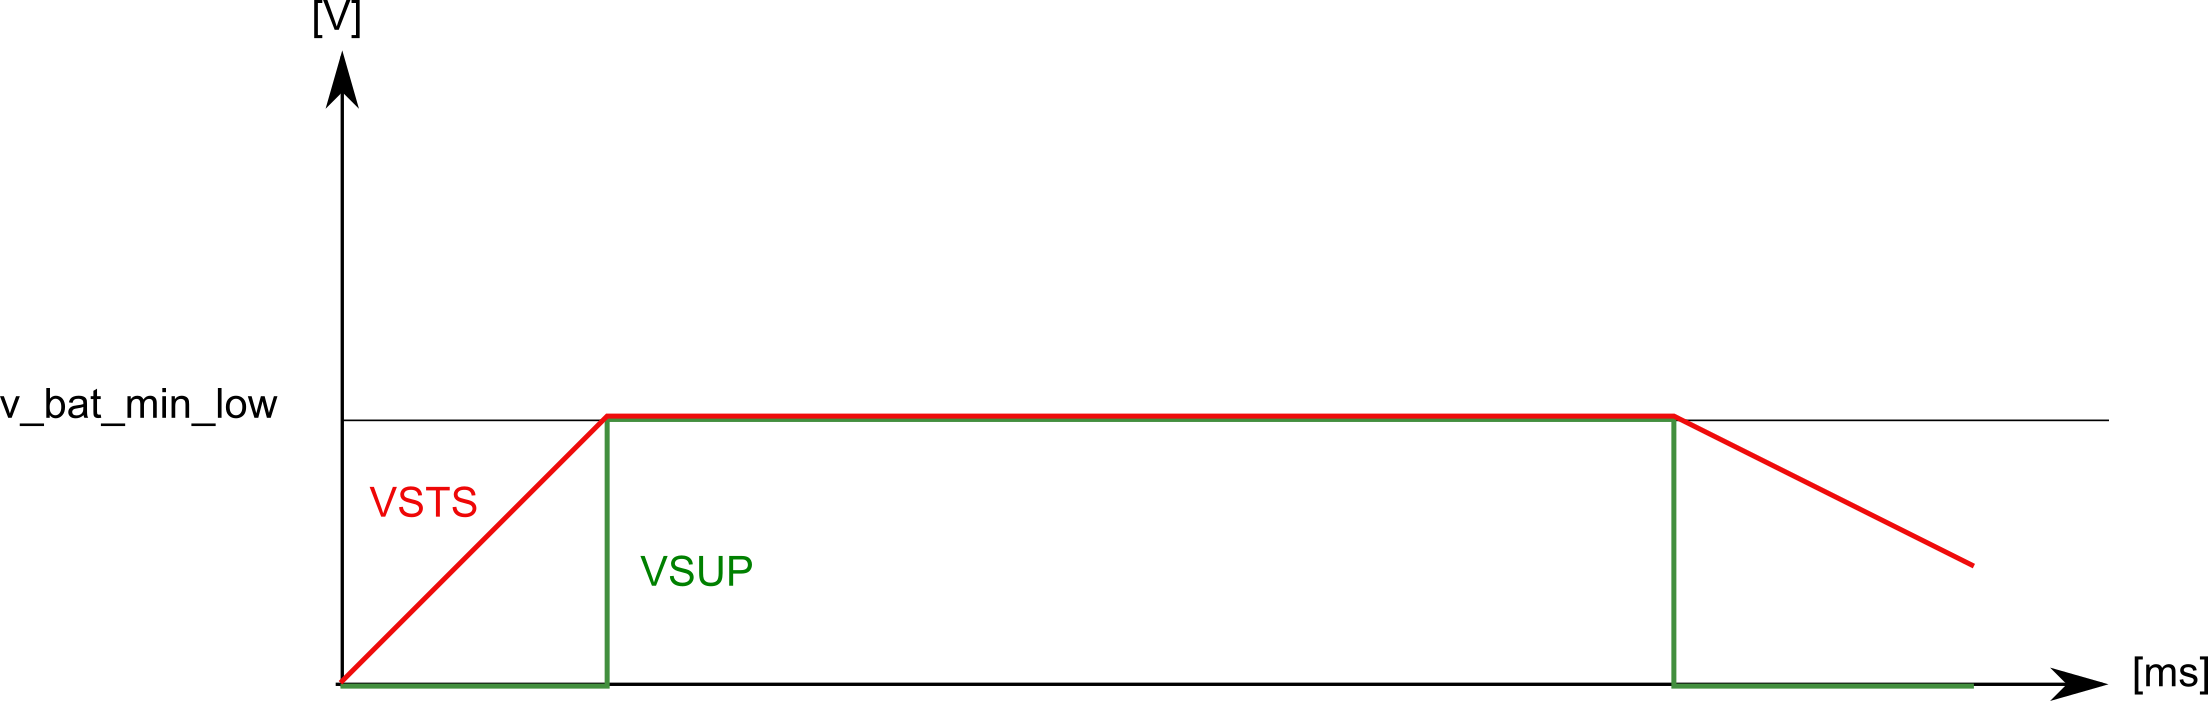
\includegraphics[width=0.9\textwidth]{2TheoretischeGrundlagen/imag/levelMitSTsTheoriel.png}
   \caption{Grundprinzip Applikationsspeisung }
   \label{em_grundprinzip} 
 \end{minipage}
 \begin{minipage}[t]{0.5\textwidth}
   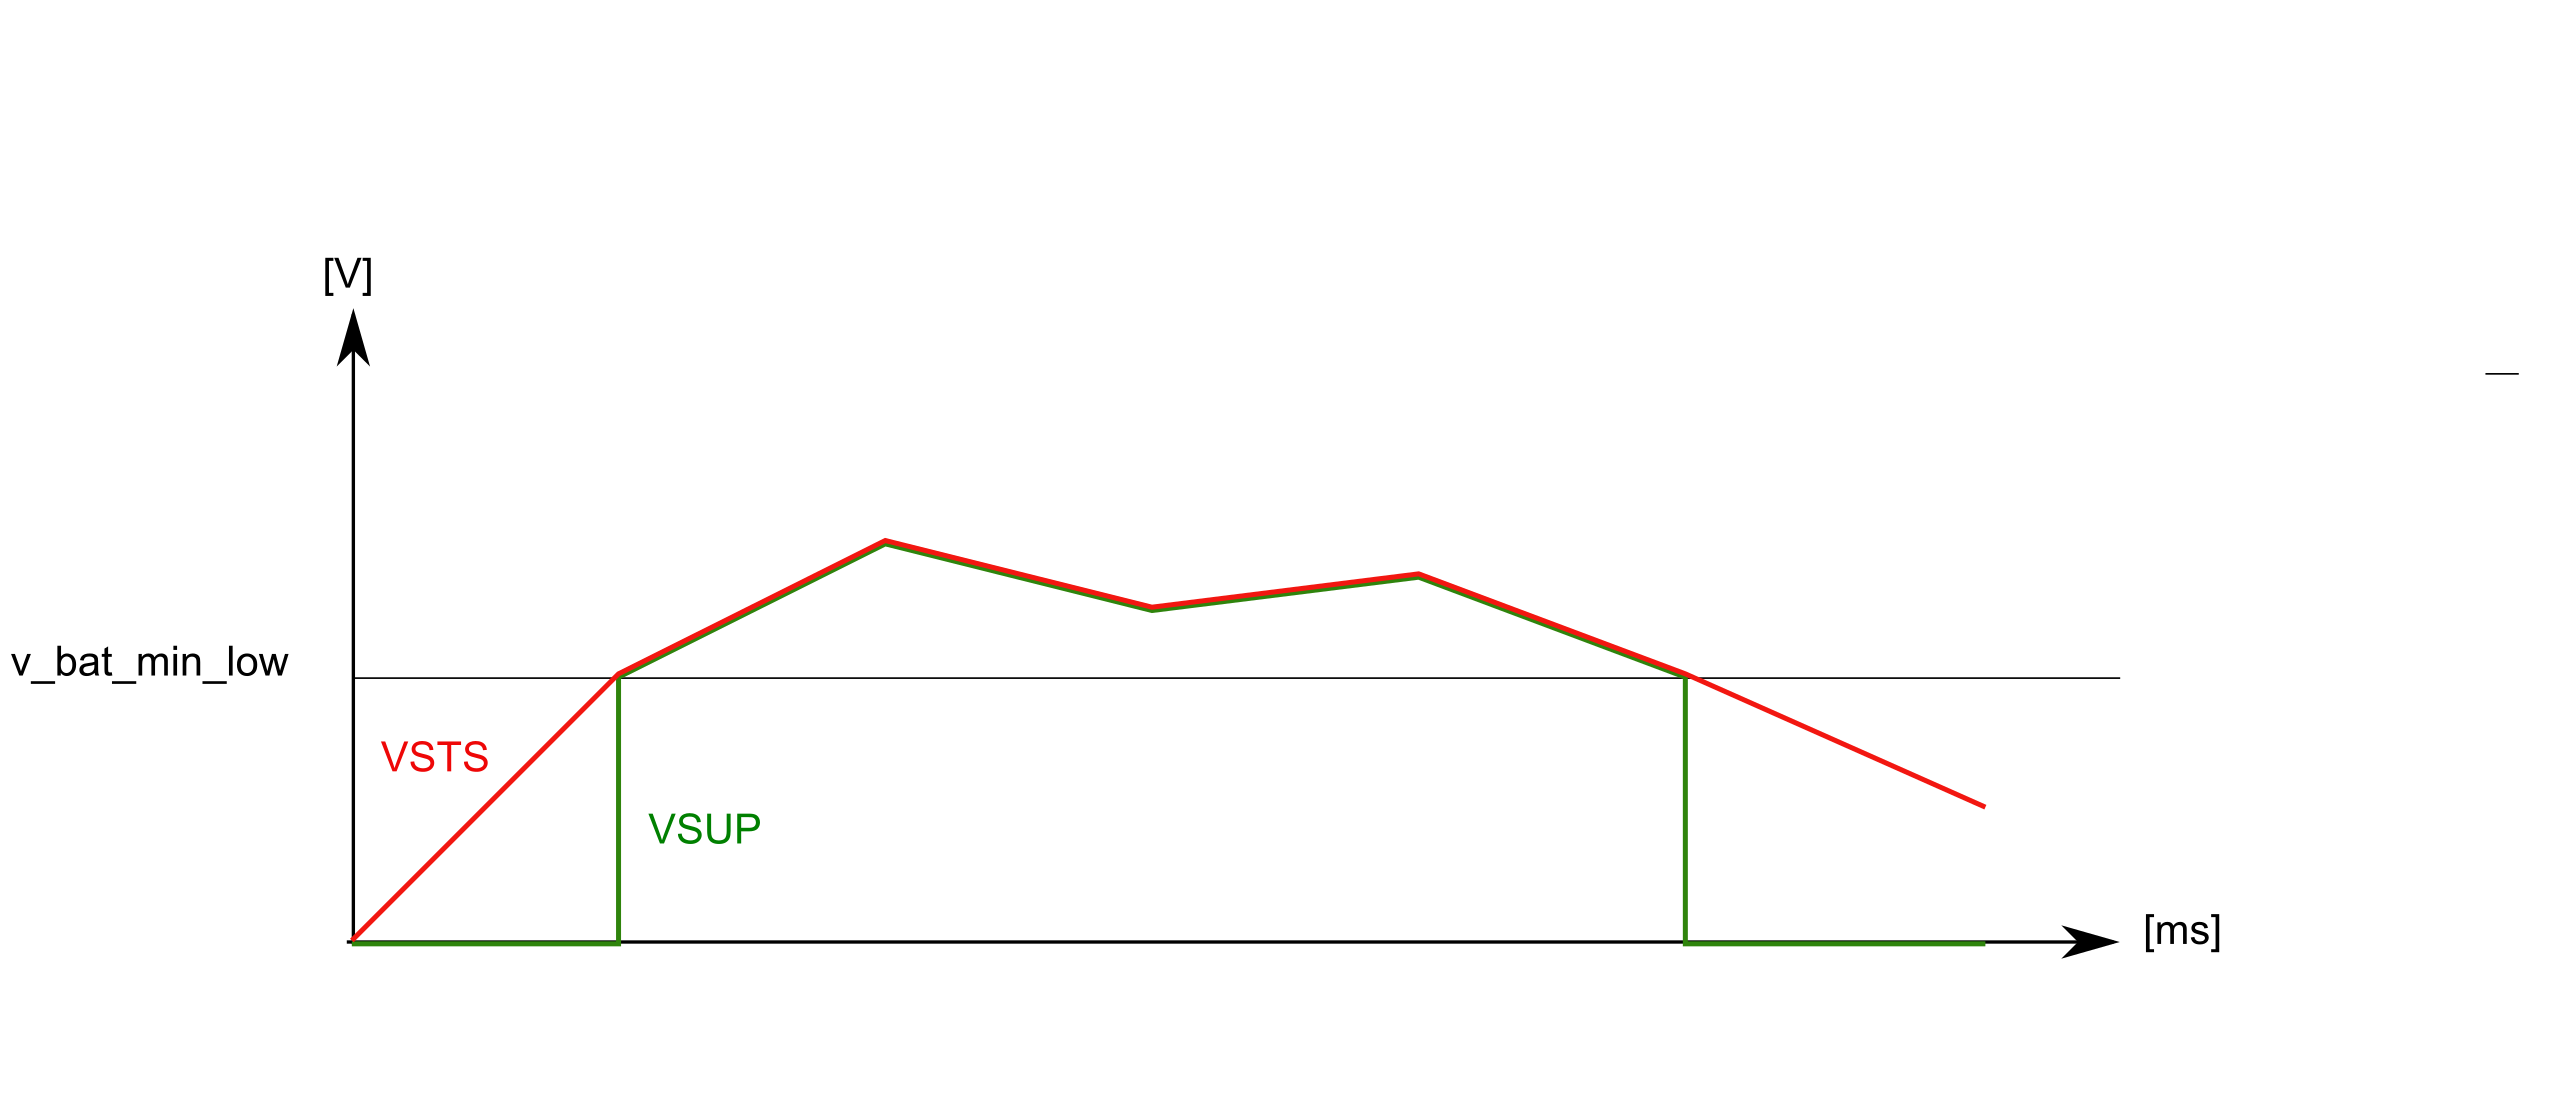
\includegraphics[width=0.9\textwidth]{2TheoretischeGrundlagen/imag/levelSTSReal.png}
   \caption{Applikationsspeisung EM8500}
   \label{em_grundprinzip_em8500} 
 \end{minipage}
\end{figure}

Im EM8500 wird dies folgendermassen umgesetzt (Abbildung \ref{em_grundprinzip_em8500}): Erreicht der Primär\-speichers STS den Schwellwert v\_bat\_min\_low, wird VSUP mit der eingestellten Spannung gespiesen. Die Applikation sollte nicht alle Energie verbrauchen, sodass sich der Speicher weiter lädt. VSUP folgt der Speicherspannung. Verbraucht die Applikation viel Energie, fallen VSUP und VSTS parallel. Speiste der Harvester viel Energie, steigt bei beiden die Spannung an. Unterschreitet VSTS/VSUP den Schwellwert von v\_bat\_min\_low, so wird die Speisung der Applikation gestoppt.



Der Primärspeicher STS ist für die kurzfristige Speisung der Applikation verantwortlich. So bedeutet STS Short Time Storage. Für das langfristige, sichere Ausführen braucht das System ein Long Term Storage (LTS). Seine Aufgabe ist, Reserveenergie aufzubauen. Diese überbrückt die Energieengpässe, wenn der Harvester zu wenig Energie liefert.
VLTS wird geladen, wenn der Schwellwert bei v\_appl\_max\_los ist (siehe Abbildung \ref{energiespeisung_lts}).

\begin{figure}[ht]
 \begin{minipage}[t]{0.5\textwidth}
   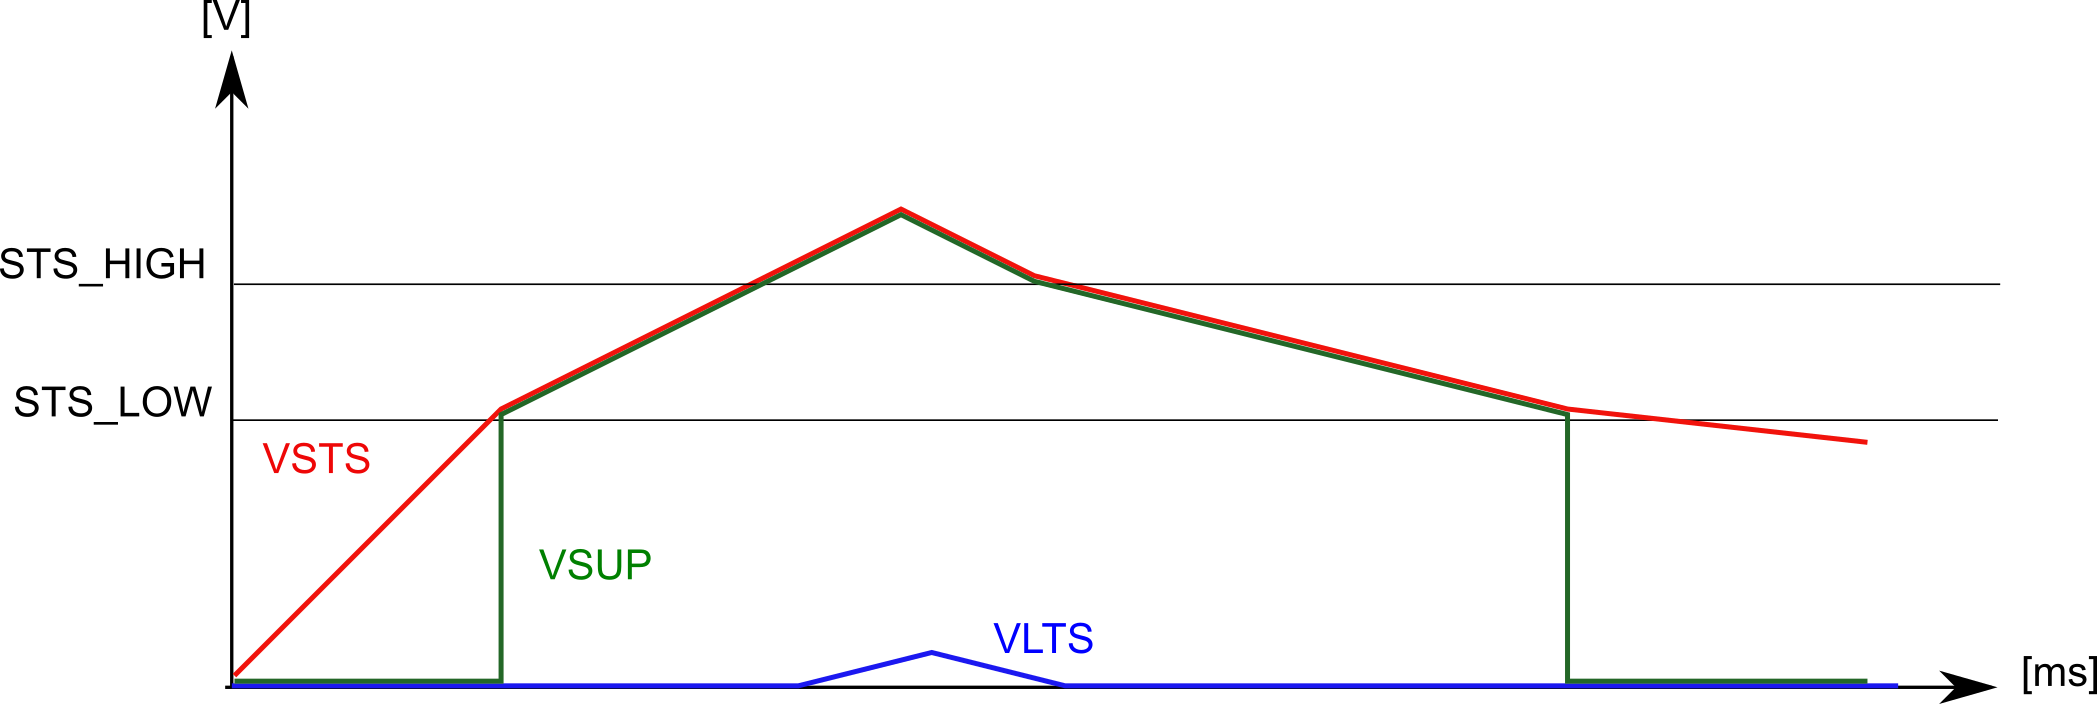
\includegraphics[width=0.9\textwidth]{2TheoretischeGrundlagen/imag/levelMitLTS.png}
   \caption{Sicheres Betreiben durch Long Term Storage}
   \label{energiespeisung_lts} 
 \end{minipage}
 \begin{minipage}[t]{0.5\textwidth}
   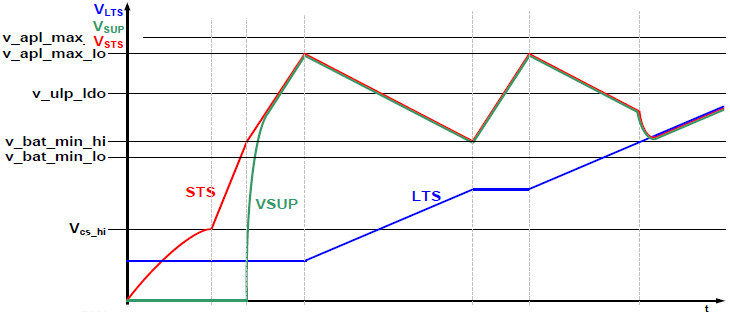
\includegraphics[width=0.9\textwidth]{2TheoretischeGrundlagen/imag/KonzeptFirma.png}
   \caption{Konzept Hersteller (\cite{datasheet_EM85})}
   \label{konzept_levels_em} 
 \end{minipage}
\end{figure}

Im Datenblatt des EM8500 (siehe \cite{datasheet_EM85}) sind weitere Feineinstellungen beschrieben und drei Application Notes helfen bei der Berechnung der Schwellwerte für ein sicheres betreiben. Die Dateien sind auf der CD abgelegt.

Grundsätzlich ist zur Berechnung der Speicher und den Schwellwerten zu sagen, dass der erste Schwellwert (v\_bat\_min\_lo), bei dem die Speisung der Applikation beginnt, genug Energie für die Initialisierung der Applikation gesammelt haben muss. Zudem muss das Abschalten von VSUP vermieden werden. Denn ein Neustart braucht aufgrund der Initialisierung viel Energie und ist ein unnötiger Kraftakt in einem Low Power System. In den Beispielkonfigurationen des Herstellers (\cite{datasheet_EM85} S. 5 - 8 ) sieht man, dass in deren Überlegungen VSUP nicht abgeschaltet wird. Der Hersteller geht davon aus, dass sogar bei dem Freischalten von VSUP die Spannung am STS nicht aufgrund der Last der Applikation fällt, sondern sich weiterhin auflädt.

\subsection{Regelung des optimalen Leistungsbezugs}
\label{optimaleLeistung}

Wichtigster Punkt in der Energieoptimierung ist, das Maximum aus der produzierten Energie weiterzuverwenden. Aus diesem Grund wird vor Inbetriebnahme eine Leistungskurve des Harvesters erstellt. Wie in Unterkapitel \ref{harv_diff} beschrieben, unterscheidet sich der Maximum Power Point (MPP) unter den Harvestern stark.

EM8500 versucht die Quelle stets in der Nähe dieses Optimums zu betreiben. Dies geschieht über eine Innenwiderstand-Regelung, sodass die Eingangsleistung möglichst dem MPP entspricht. Wie schnell die aktuelle Leistung überprüft wird, ist einstellbar. Der EM8500 besitzt eine Auflösung von 37 mV. Die Abbildung \ref{RegelungSpannung} zeigt das periodische Messen des Spannungswert des Harvesters. Da die Kurzschlussmessung für das Messen des Stromwerts eine Spannungsspitzen verursacht, (gut zu sehen in der Abbildung bei höherer Spannung), sollte die Leistungsüberprüfung nicht zu oft geschehen. Spannungsspitzen bedeuten Energieverlust, weshalb die Energiemessung nur so oft als  absolut notwendig erfolgen soll. In der Abbildung \ref{RegelungSpannung} beträgt die Periode 8 s. 

\begin{figure}[ht]
    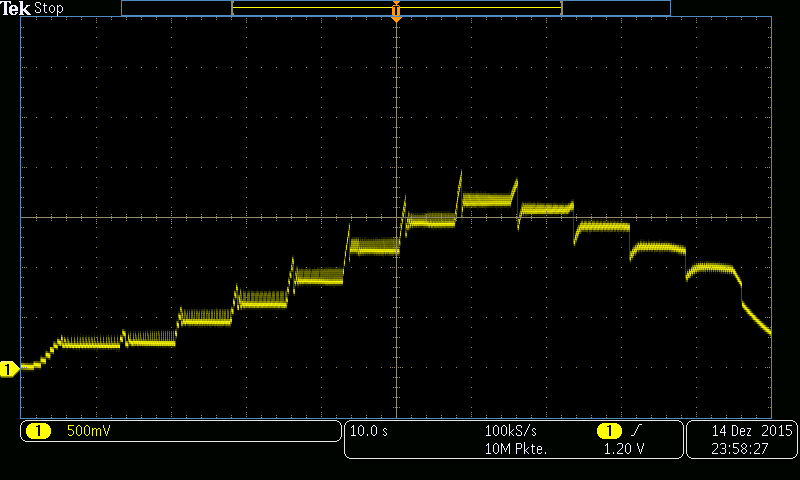
\includegraphics[width=0.5\textwidth]{2TheoretischeGrundlagen/imag/RegelungVHRV.png}
    \caption{Leistungsmessung des Harvesters}
    \label{RegelungSpannung} 
\end{figure}


\subsection{Booster definiert Spannung}
\label{eingangsspannung}

Direkt mit dem MPPT-Kontroller ist der Booster (siehe Blockdiagramm im Anhang \ref{anhang_em8500}). Die Aufgabe des Boosters ist es, das interne Spannungsniveau (VREG) zu heben. Der Booster arbeitet ab einer Eingangsspannungen von 0.3 V. Danach regelt er in Schritten von 0.3 V. Der Booster geht von einer Gleichspannung eines TEG oder einer Solarzelle aus. Für diese zwei Anwendungen ist der EM8500 konzipiert (siehe \cite{datasheet_EM85}, Abschnitt Description, S.1).


\subsection{Energiezustand kennen und In- und Ausgänge schalten}
\label{th_energiebilanz}

Da der Primärspeicher STS vom Boosterausgang $V_{Booster}$ gespiesen wird, entspricht dessen Spannung dem des Boosterausgangs. $E_{Applikation}$ bezeichnet die  minimale Energie, die die Applikation braucht, also mindestens die Initialisierung der Applikation. 

\begin{equation}
  E_{Applikation}= C_{STS} \times \frac{1}{2}\, (V_{Booster} )^2
\end{equation}

Da sich der Kondensator $C_{STS}$ bei der Freigabe der Energie über V\_SUP nicht auf 0 entlädt, sondern die minimale Applikationsspannung erhalten bleibt, gilt für die Berechnung des Kondensators $C_{STS}$ nur die Energiedifferenz als verwendbar. Es ist die Differenz zwischen den zwei eingestellten Primärspeicher-Schwellwerten v\_bat\_min\_hi\_dis (ab da wird V\_SUP gespiesen) und  v\_bat\_min\_low (ab da hört die Speisung von V\_SUP auf). Die zwei Schwellwerte werden in der Gleichung vereinfacht als STS\_HIGH und STS\_LOW bezeichnet.

\begin{flalign}\label{eq:e-high-e-low}
E_{Applikation} &= E_{STS\_HIGH} - E_{STS\_LOW}\\\nonumber
                &= C_{STS} \times \frac{1}{2}\, (V_{STS\_HIGH} )^2 - C_{STS} \times \frac{1}{2}\, (V_{STS\_LOW} )^2
\end{flalign}
%\eqref{eq:e-high-e-low} % with brackets
%\ref{eq:e-high-e-low} % look ma no  brackets

Kennt man die notwendige Energie, so kann die Grösse des Kondensator $C_{STS}$ aus der notwendigen Energie berechnet werden:

\begin{equation}
  C_{STS}= \frac{ E_{Applikation}}{(V_{STS\_HIGH} )^2 - (V_{STS\_LOW} )^2}
\end{equation}

Umgekehrt argumentiert, kann man aus der Höhe der Applikationsspannung (V\_SUP bzw. $V_{STS\_LOW}$), des bekannten Energiekonsums $E_{Applikation}$ den notwendigen Schwellwert für den Primärspeicher berechnen:

\begin{equation}
(V_{STS\_HIGH}) ^2 - (V_{STS\_LOW})^2 =  \frac{2\, \times \, E_{Applikation}}{C_{STS}}
\end{equation}


\begin{equation}
(v\_bat\_min\_low) ^2  =  \frac{2\, \times \, E_{Applikation}}{C_{STS}} + (V_{STS\_LOW})^2
\end{equation}




Neben VSUP kann der EM8500 drei weitere Ausgänge freischalten: VAUX[0] bis VAUX[2] (siehe Abbildung  \ref{IOEM8500}). Vor allem aber kann per I2C oder SPI der aktuelle Spannungspegel der Regelung (VREG), die Speicher (VDD\_STS und VDD\_LTS)und des Harvestereingangs (VDD\_HRV) abgefragt werden. So kennt die Applikation jederzeit den aktuellen Energiezustand der gesammelten Energie.

EM8500 stellt zwei digitale Überwachungssignale zur Verfügung:\\ 
Der Ausgang HRV\_LOW ist auf logisch '0', wenn die Eingangsspannung vom Harvester grösser als 0.3 V ist. Fällt diese darunter, geht HRV\_LOW auf logisch '1'.
Der Ausgang BAT\_LOW zeigt die Zeitdauer an, in der nur STS die Applikation speist:

\begin{itemize}
     \item BAT\_LOW = '0'\\
           Nicht genügend Energie zur Speisung der Applikation.
           VSUP ist ausgeschaltet.
     \item BAT\_LOW = '1'\\
           Genügend Energie zur Speisung der Applikation.\\
           VSUP ist eingeschaltet.
      \item BAT\_LOW = '0'\\
           Genügend Energie zur Speisung von LTS.\\
           VSUP ist eingeschaltet.\\
           Der Zustand entspricht nicht mehr BAT\_LOW.   
\end{itemize} 

Mit den zwei digitalen Signalen kann der Energiezustand grob abgebildet werden.

\begin{figure}[ht]
    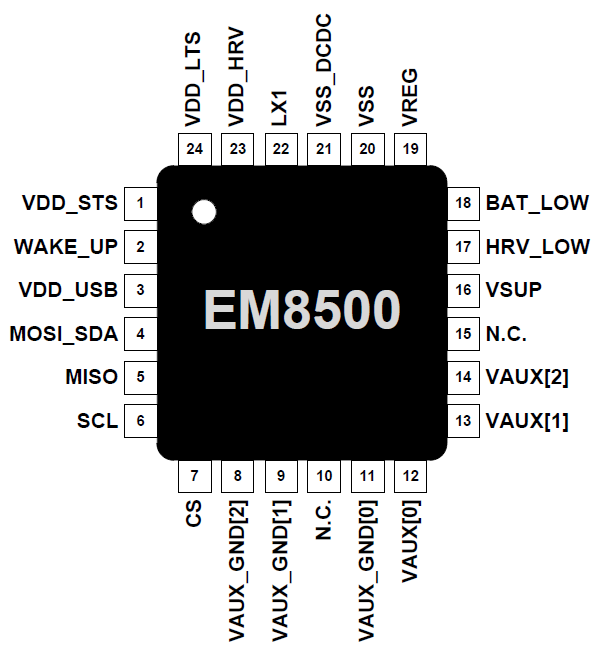
\includegraphics[width=0.5\textwidth]{2TheoretischeGrundlagen/imag/EM8500IO.png}
    \caption{In- und Outputs EM8500  (\cite{datasheet_EM85}, p.11)}
    \label{IOEM8500} 
\end{figure}


%$\bar{E_{HRV}} \ge \bar{E_{BLE}} $
%Die Energie der Quelle [$\bar{E_{HRV}} $] muss ausreichen für das Versenden der Datenpakte über Bluetooth smart [$\bar{E_{BLE}}$].
%
%\[\bar{E_{HRV}} = \bar{P} * t \ge \bar{E_{BLE}}  \]
%\[\bar{P_{10km/h}} * t = 11 * 10^{-3}  \]
%\[74.4 * 10^{-6} * t = 11 * 10^{-3}   \]
%\[t = 147 s  \]
%
%\[\bar{E_{HRV}} = \bar{P} * t \ge \bar{E_{BLE}}  \]
%\[\bar{P_{10km/h}} * t = 11 * 10^{-3}  \]
%\[74.4 * 10^{-6} * t = 11 * 10^{-3}   \]
%\[t = 147 s  \]

% 2.3-------------------------------------------------------

\section{Power Management}\label{t_power_management} 

Die Aufgabe des EM8500-Chip ist es, Energie zu sammeln und kontrolliert frei zu geben. Die Aufgabe das nachfolgenden Microkontrollers ist es, die freigegebenen Energieportionen optimal zu verwenden. Das bedeutet, möglichst wenig Energie bei der Datenverarbeitung zu benötigen. Dies wird durch Abstellen aller unnötigen Microkontroller-Bereiche erreicht und einem zusätzlichen Schlafen während allen Warteprozessen.

In diesem Kapitel werden drei Konzepte zum Umsetzen eines Low Power Systems vorgestellt. Das Hauptthema ist das Schlafen zwischen allen Prozessen. Dies wird im ersten Unterkapitel beschrieben. Das Schlafen bedingt ein Aufwecken aufgrund von Ereignissen. Dadurch ergibt sich eine Interrupt Driven Applikation. Diese wird im zweiten Unterkapitel erklärt. Als letztes dient ein Design Aspekt: Durch das Einbauen einer State Machine über alle laufenden Interrupts, ist es nachfolgenden Entwicklerinnen und Entwicklern einfacher, den Code und die gegenseitigen Beeinflussungen zu verstehen. Dies wird im Unterkapitel beschrieben.

Vor der technischen Beschreibung der Konzepte in den drei Unterkapiteln wird kurz auf die verwendete Hardware eingegangen. In der Bachelorarbeit war als Microkontroller das Simple Link TI-SensorTag von Texas Instrument vorgegeben. Der Grund für dieses Board ist, dass das TI-SensorTag drei Anforderungen auf einem Board vereint:

\begin{itemize}
    \item Ein Cortex M3 dient als Haupt-Microkontroller und ist aufgrund seiner hohen, und somit schnellen, Rechenleistung und seiner Low Power-Fähigkeiten für eine Harvester-Anwendung wie der Bicycle Computer geeignet.
    \item Auf dem Board ist ein zweiter Cortex M0 für die Wireless-Anbindung angeschlossen. Dieser Prozessor kann von der Benutzerin oder dem Benutzer nicht programmiert werden, da die Schnittstelle zur Low Power Datenkommunikation fix aufgesetzt ist. Neben Bluetooth Low Energy kann auch Zigbee verwendet werden.
    \item Auf dem Board sind 10 Sensoren angebunden.
\end{itemize}

Die Funktionsblöcke des TI-SensorTags befinden sich im Anhang \ref{anhang_sensortag}.

\subsection{Einbauen von Schlaufmodi}\label{pm_sleep} 

(Low Power Microcontroller können Gebiete des Prozessors oder von Peripherieelementen temporär ausschalten. Das System befindet sich im Standby Modus. Nur die für die Applikation unabdingbaren Aktivitäten laufen mit niederstem Takt weiter. Über Interrupts können einzelne Bereich aufgeweckt werden, die ihre Aktionen ausführen und danach geht das System wieder in den Standby Modus.)


Dass Prozessoren nach längerer Zeit ohne externen Input in den Schlafmodus gehen, ist Usus (Allgemeingut, bekannt). Bei einer Low Power Applikation geht der Prozessor jedoch nach kleinsten Ausführungsblöcken direkt wieder schlafen. So gehört zu jedem Aufwecken einer Peripherie, der Parallele Schlafmodus, bis dass die Peripherie gestartet ist. (Dies gilt auch für die Sensoren.) In diesem Unterkapitel werden zwei Umsetzungen des Sleep-Moduses konzeptionell erklärt.

\subsubsection{Schlafen zwischen Ausführungen}
\label{schlafen_theorie}

Die Abbildung \ref{sleep_Grundprinzip} zeigt das Grundprinzip. Das Programm besteht aus verschiedenen Aktionsblöcken. Diese dauern unterschiedlich lang und verbrauchen unterschiedlich viel Energie. Zwischen den Aktionen ist eine frei wählbare Wartezeit einbaubar ($\Delta$ t0 - t3). Die graue Markierung in jedem Aktionsblock sind die Initialisierungen vor jeder Aktion.

Während der Schlafenszeit sind alle Peripherien abgeschaltet und im Prozessor (hier als Bsp. Cortex M3) wird nur die Konfigurationen im Flash regelmässig \glqq refreshed\grqq. (Zu den unabdingbaren Aktivitäten eines laufenden Microkontrollers gehört das Refreshen (Neuladen) der Register mit den Systemeinstellungen. Diese Refreshing-Peaks sieht man im Standby Modus.)  Dies ist in der Abbildung \ref{sleep_Grundprinzip} an den grünen Spannungsspitzen zu sehen. Ohne "refreshen" des Speichers, gehen die Konfigurationen verloren und vor jeder Aktion muss das System neu komplett initialisert werden.

\begin{figure}[ht]
    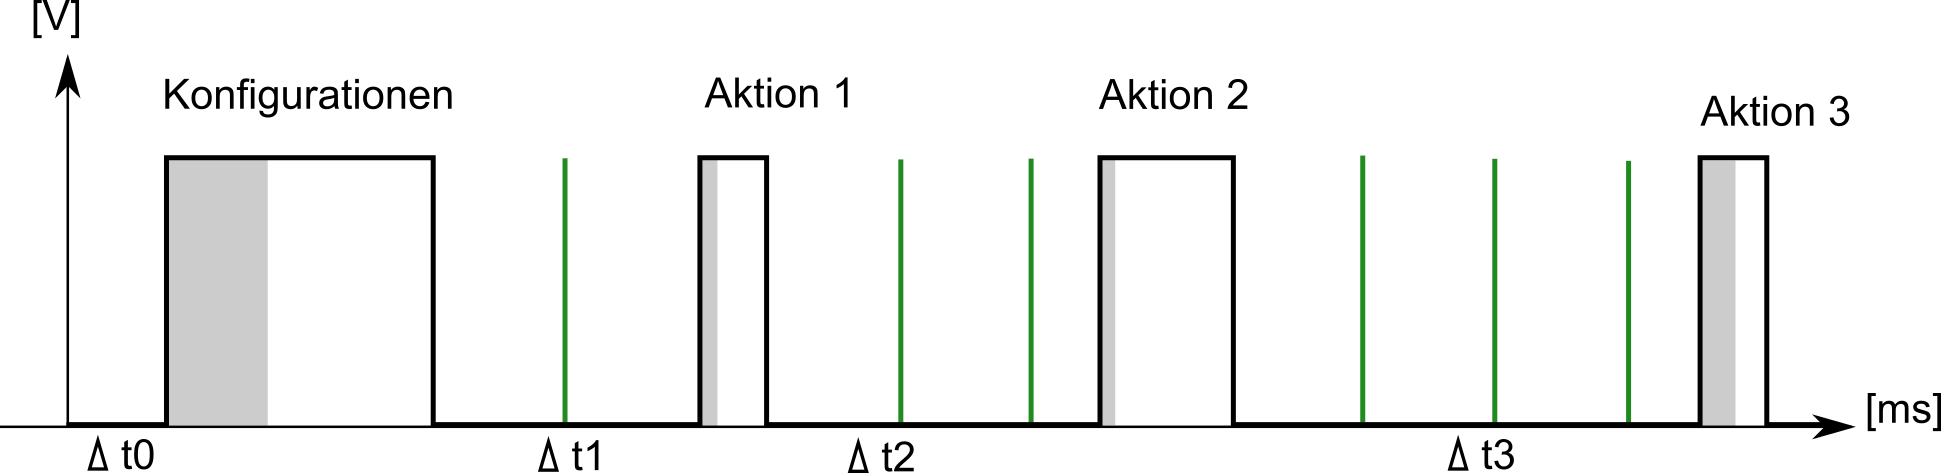
\includegraphics[width=\textwidth]{2TheoretischeGrundlagen/imag/SleepGrundprinzip.png}
    \caption{Schlafen zwischen Ausführungen}
    \label{sleep_Grundprinzip} 
\end{figure}

\subsubsection{Schlafen innerhalb einer Aktion}
Bei einer Applikation im $\mu$ - oder mW-Bereich wird bei jedem Warteprozess, wie z.B. die Zeit, die der Sensor zum Aufwachen braucht, in den Sleep-Mode gegangen. Innerhalb des Codes dominieren die Aufwach- und Abstelleinstellungen. Für jede Aktion, wird nur die PowerDomain dieser Funktionalität eingeschaltet und nach ausführen der Aktion wieder abgeschaltet. Die Abbildung \ref{sleep_intern} zeigt dieses Prinzip mit UML dargestellt.

\begin{figure}[ht]
    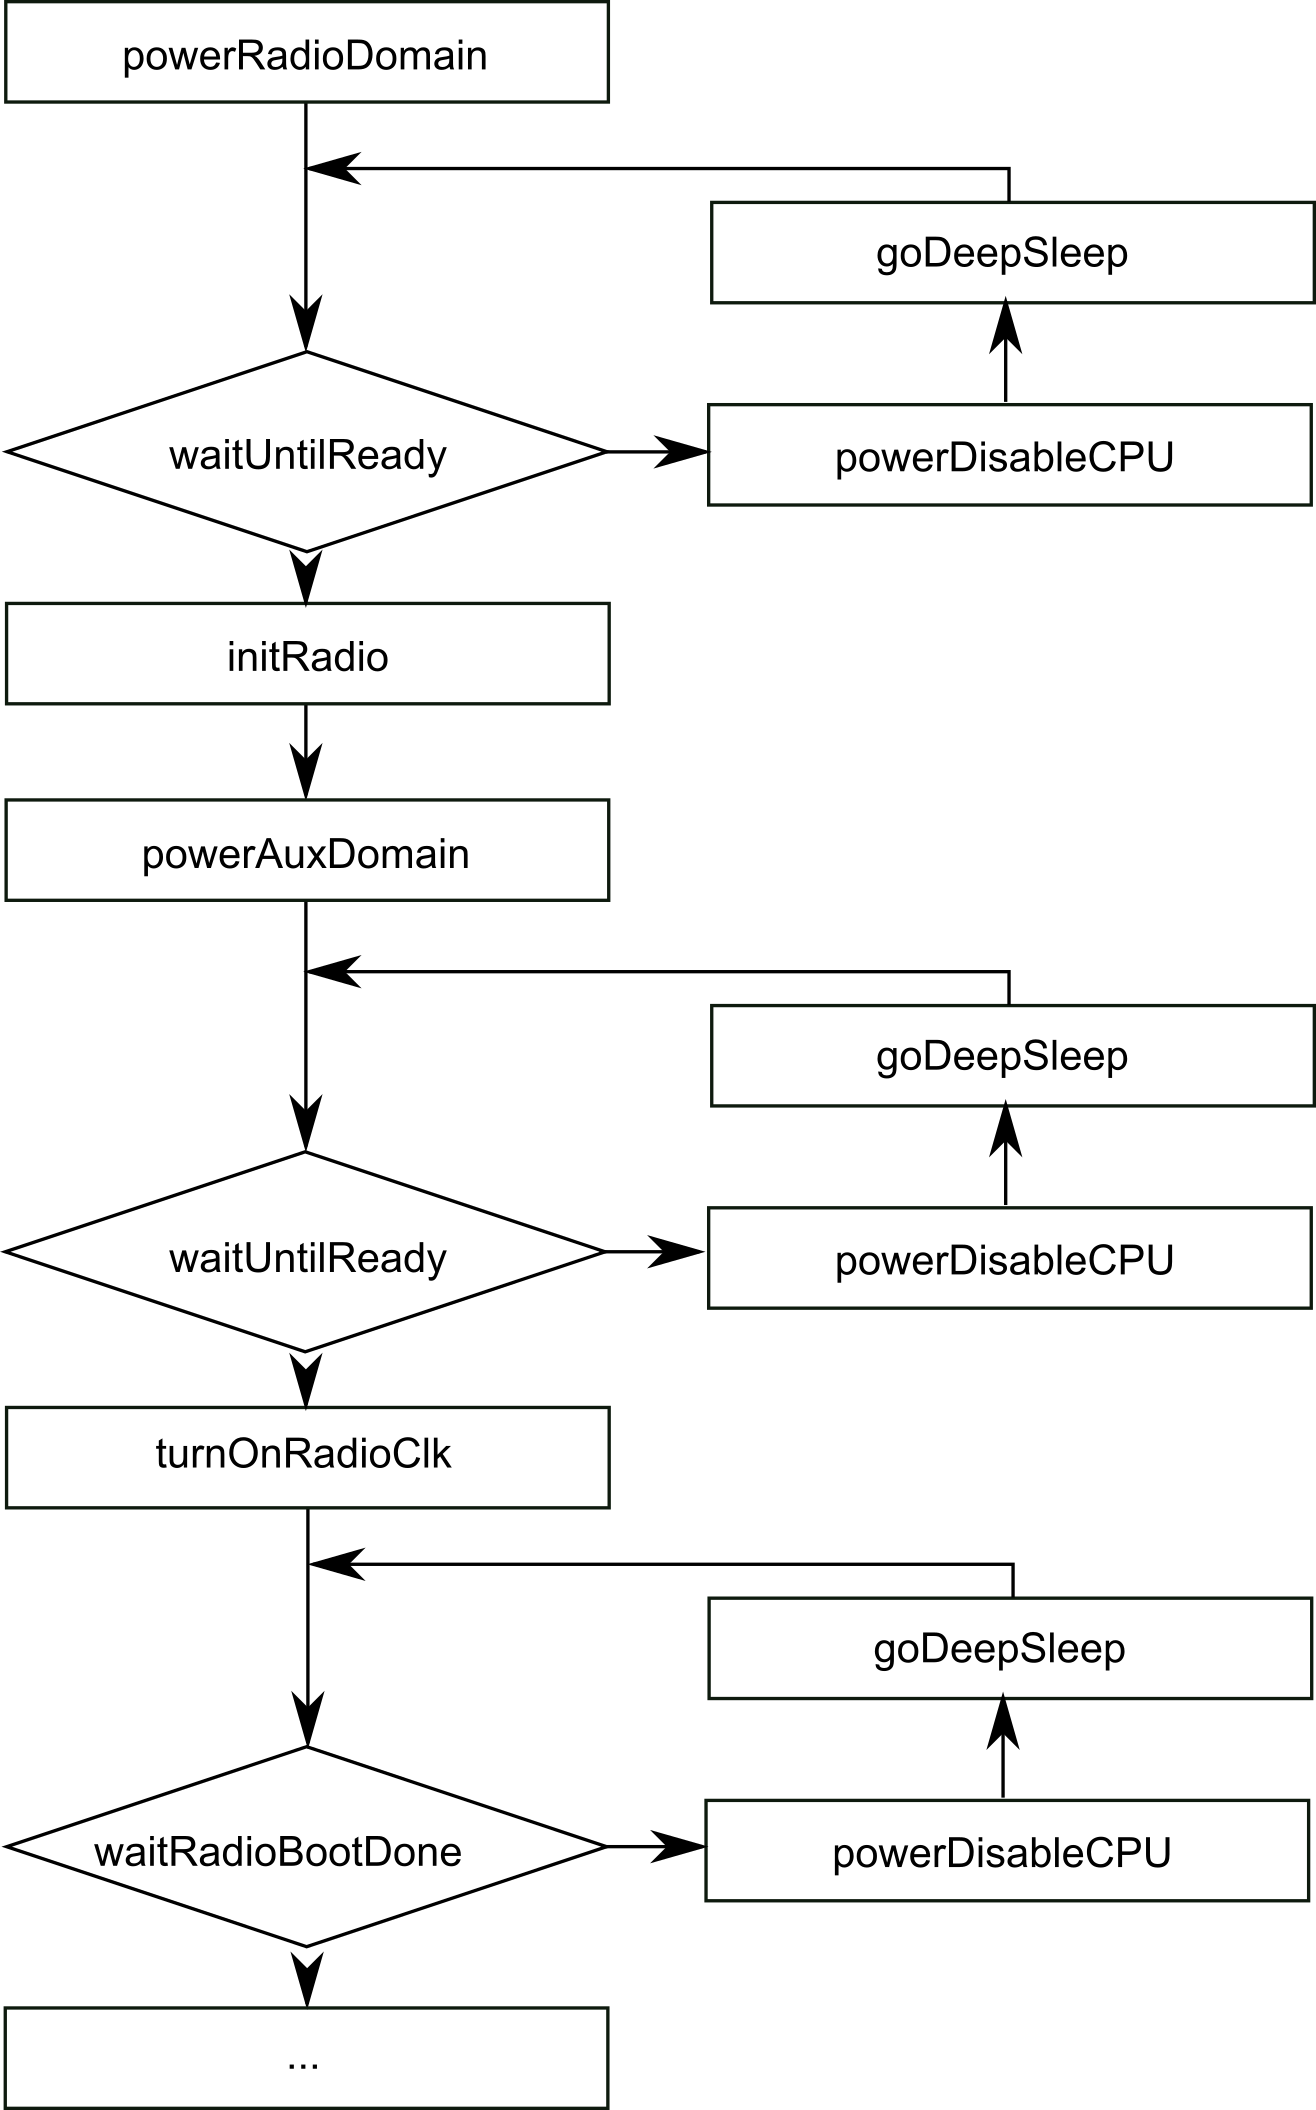
\includegraphics[width=0.5\textwidth]{2TheoretischeGrundlagen/imag/SleepInFunktion.png}
    \caption{Schlafen innerhalb des Codes}
    \label{sleep_intern} 
\end{figure}


\subsection{Interrupt Driven Application}\label{pm_interrupt} 
Zum Schlafen gehört auch ein Aufwachen. Dies ist ein nicht-triviales Problem, lässt sich mit Interrupts lösen. In diesem Unterkapitel werden zwei Konzepte einer Interrupt Driven Applikation erklärt: fixes Aufwachen aufgrund interner Interrupts und asynchrones Aufwachen aufgrund externer Events.

\subsubsection{Aufwachen durch interne Interrupts}
Ein System kann intern seine Signale auswerten und aufgrund kombinatorischen Logik, dem erreichen eines Schwellwerten oder dem Ablaufen eines Timers aufwachen. Solche Wakeups sind fix und unabhängig von äusseren Einflüssen. Ein System mit internen Interrupts ist determinierbar. Das heisst, der Empfang interner Interrupts ist präzis (nur 1 malig und kein Prellen) und kann über Prioritäten gut geregelt werden.

\subsubsection{Aufwachen durch externe Events}
Der Prozessor, oder Teile davon, können auch aufgrund äusserer Impulse aufwachen. Die Verarbeitung des Interrupts ist dieselbe, nur weiss man nicht, wann das Ereignis auftritt. Die Gefahr, dass zwei Interrupts zur selben Zeit eintreffen oder eine Quelle mehrere Interrupts sendet, ist gegeben. Das Löschen der eingegangenen Interrupts und das Prüfen, ob ein Event nicht zu oft verarbeitet wird, muss bewerkstelligt werden. Löst eine Quelle Interrupts über längere Zeit aus, kann dies das System absorbieren und schlimmstenfalls den Systemablauf aus dem Rhythmus bringen.

%\subsection{State Machine für definierte Abläufe}\label{pm_state_machine} 
%Low Power Applikationen enthalten viele Interrupts. Jede grössere Tätigkeit braucht das Aktivieren mehrerer Schnittstellen, die alle aufgeweckt und aufeinander abgestimmt werden. Da die Codeausführung nicht sequentiell verläuft, sondern Ausführungen in den Interrupt-Handlern stehen, ist ein Überblick der Abhängigkeiten nicht einfach ersichtlich. Um unerwünschte Effekte zu vermeiden, kann eine State Machine implementiert werden. Diese stellt sicher, dass nur aufgrund von gewissen Signalen, ein Aktion ausgeführt wird. Alle anderen Effekte werden ignoriert. Die Abbildung \ref{t_stateMachine} zeigt die definierte Abhängigkeiten durch eine State Machine.
%
%\begin{figure}[ht]
%    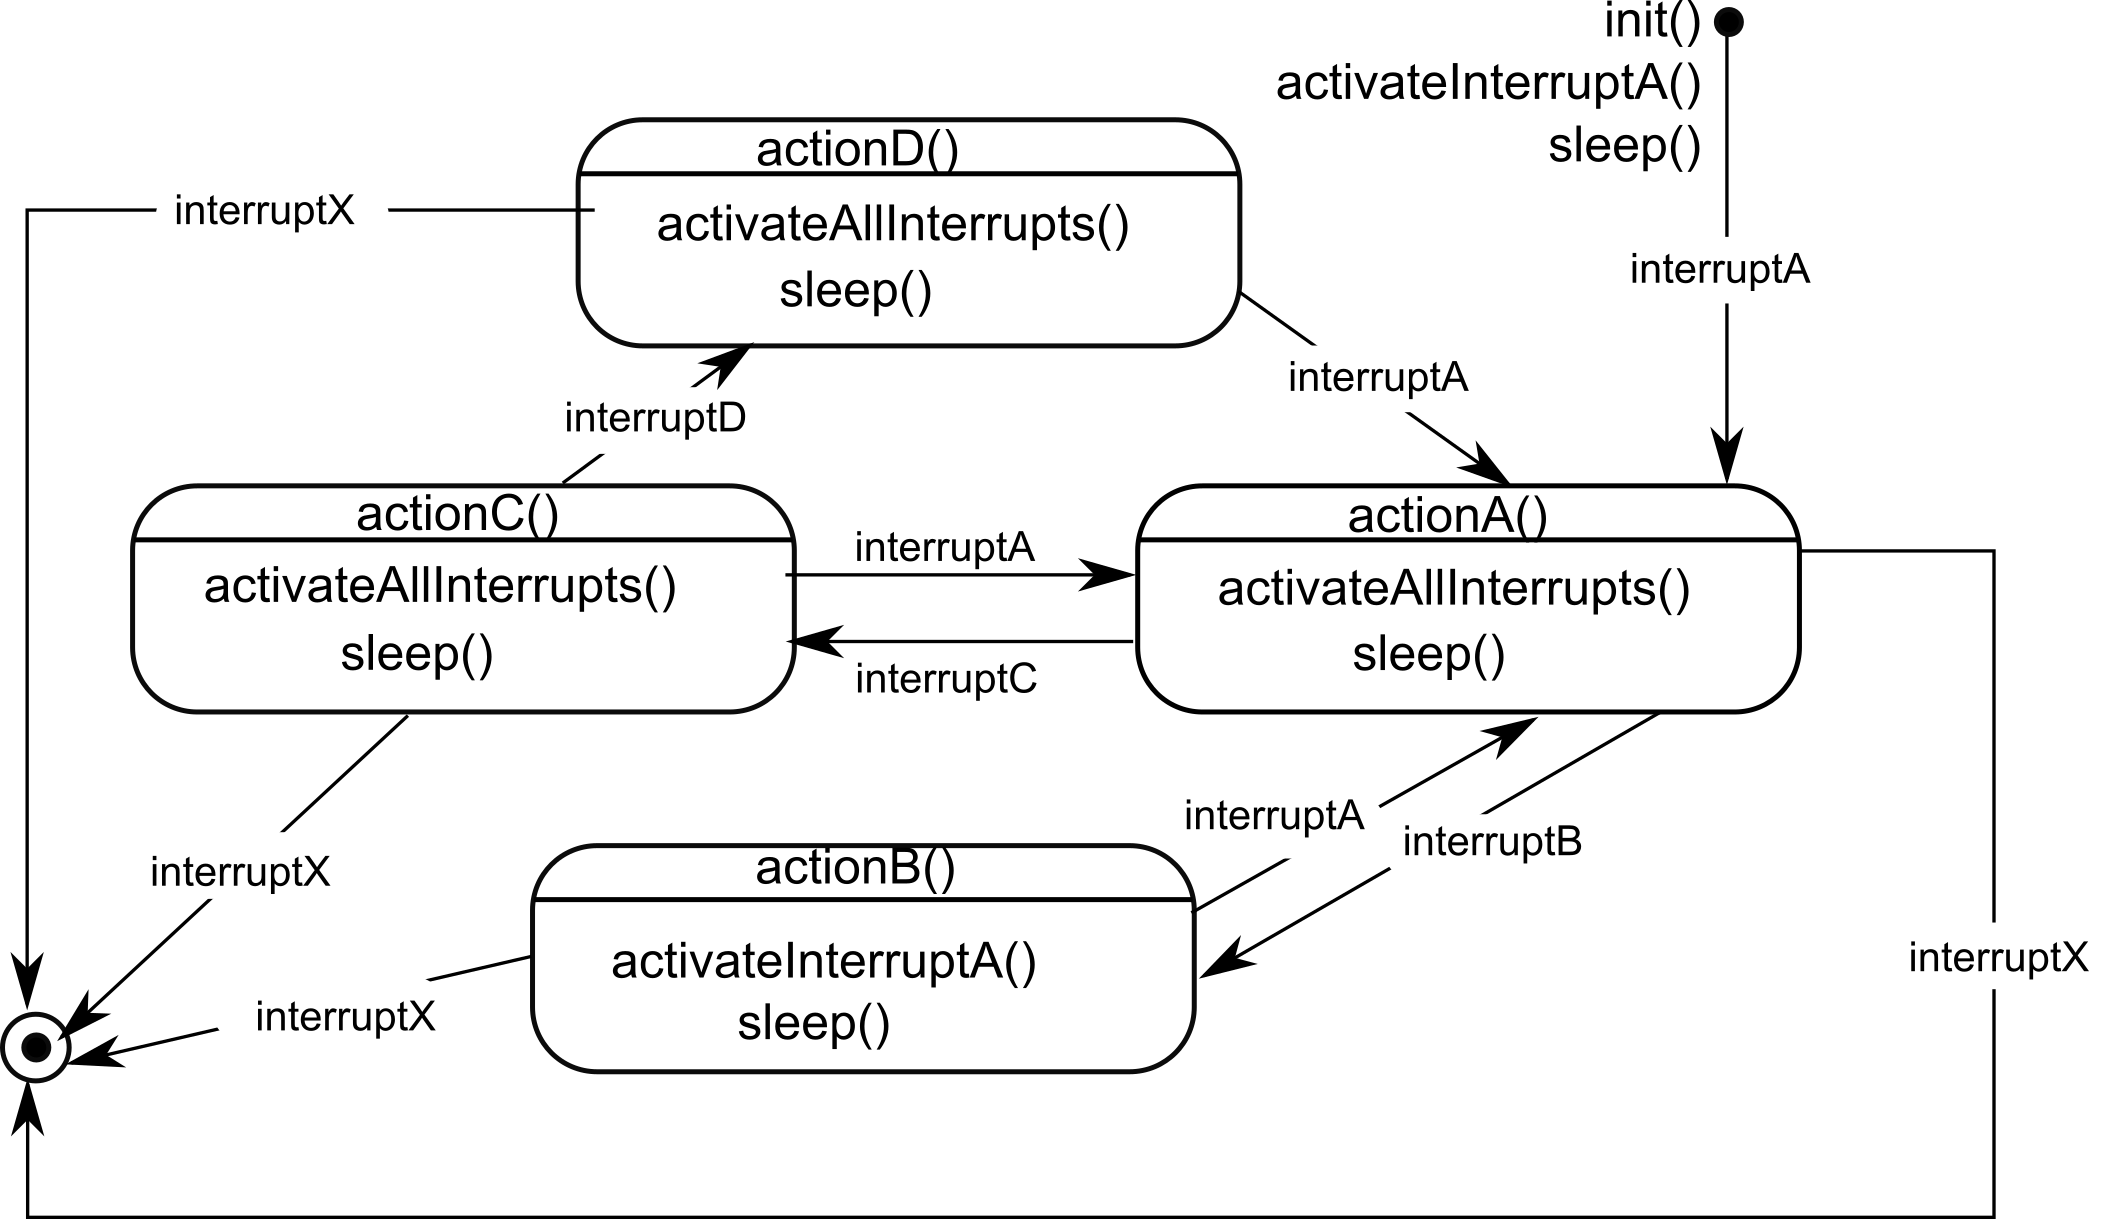
\includegraphics[width=1.0\textwidth]{2TheoretischeGrundlagen/imag/StateMachineGrundlage.png}
%    \caption{Struktur durch State Machine}
%    \label{t_stateMachine} 
%\end{figure}

% 2.4-------------------------------------------------------------------
\section{Bluetooth Low Energy}\label{t_ble} 

Bluetooth Low Energy (BLE) bezeichnet eine Funktechnik, welche es ermöglicht, Daten zwischen Geräten auszutauschen. Der Vorteil von Bluetooth Low Energy ist der niedrigere Energieverbrauch im Gegensatz zum traditionellen Bluetooth. Das Bluetooth Low Energy Protokoll gehört zum Bluetooth Core Specification Version 4.0, wo auch das Classic Bluetooth Protokoll und das Bluetooth High Speed Protokoll enthalten sind. Die Bluetooth Core Specification Version 4.0 ist besser unter dem Namen Bluetooth Smart bekannt und wurde im Juli 2010 veröffentlicht (\cite{youtube_BLE}).

\subsection{BLE im Vergleich zu Bluetooth}
  
Bluetooth Low Energy verwendet das gleiche Frequenzband wie das traditionelle Bluetooth, jedoch sind nur 40 Kanäle à 2 MHz verfügbar, anstatt 79 Kanäle à 1 MHz beim traditionellen Bluetooth. Ausserdem verbraucht BLE, wie der Name bereits indiziert, weniger Energie als andere Übertragungsmedien. So sendet BLE mit maximal 10 mW, was einer Reichweite von ca. 10 Metern entspricht im Gegensatz zu Klasse 1 Bluetooth-Geräten, welche mit 100 mW eine Reichweite von rund 100 Metern erreichen. Ein der BLE-Technik ist, dass die Bauteile für eine BLE-Kommunikation relativ günstig sind und damit die Geräte ebenfalls günstiger hergestellt werden können (\cite{Interent_BLE}, Abschnitt Bluetooth Range).

\subsection{Advertising und Connected Mode}
BLE wird vor allem für batterielose Sensoren verwendet, welche die Energie aus der Umwelt beziehen. Diese Sensoren arbeiten meist als Beacon, was bedeutet, dass sie Daten senden, ohne eine aktive Verbindung mit einem Gerät aufzubauen oder nur eine Verbindung auf Anfrage eingehen, diese jedoch nach kurzer Zeit wieder beenden. Dieser Modus nennt sich Advertising Mode, was vom Englischen advertisement stammt, es soll aussagen, dass der Beacon eine Werbung aussendet und diese nicht auf eine spezielle Person zugeschnitten ist, sondern an die breite Masse gesendet wird.

Eine aktive Verbindung ist bei den meisten Sensoranwendungen auch nicht notwendig, da die Daten einfach gesendet werden können und das empfangende Gerät entscheidet was mit den vorliegenden Daten gemacht wird, wenn das Gerät mehr Informationen benötigt kann eine Verbindung aufgebaut werden. Trotzdem kann mit BLE eine aktive Verbindung eingerichtet werden, jedoch verbraucht eine aktive Verbindung mehr Energie, da Daten gesendet und empfangen werden müssen. Das bedeutet der Sensor kann nicht in einen Standby- Modus gehen, in welchem weniger Energie verbraucht wird, da auf ankommende Daten gewartet wird (\cite{BLE_advertising},\cite{ELKO_BLE}).

\subsection{BLE Pakete}

Der Aufbau eines BLE Pakets ist überschaubar. Als erstes wird ein Preamble, bestehend aus abwechselnden 1 und 0, womit der Empfänger sich auf die richtige Frequenz synchronisieren kann. Diese Preamble wird auf dafür verwendet die Verstärkung des Empfängers einzustellen, dies kann sehr wichtig sein bei Signale, welche von einer grösseren Distanz versendet werden, da eine falsche Verstärkung des Signals in Fehlern resultieren kann.

Anschliessend wird die Access Address verschickt, anhand dieser Adresse kann der Empfänger die Nachricht einem ganz bestimmten Sender zuordnen und somit entscheiden, ob die Daten vom richtigen Sender kommen oder ob es eventuell nur Störungen waren, welche zufälligerweise eine Preamble dargestellt haben.

Der Header enthält Informationen zum Aufbau der Daten, welche folgen. Es gibt sieben verschiedene Arten von Aufbauten der Daten.

\begin{itemize}
    \item ADV\_IND – general advertising indication
    \item ADV\_DIRECT\_IND – direct connection indication
    \item ADV\_NONCONN\_INC – nonconnectable indication
    \item ADV\_SCAN\_IND – scannable indication
    \item SCAN\_REQ – active scanning request
    \item SCAN\_RSP – active scanning response
    \item CONNECT\_REQ – connection request
\end{itemize}

Nachfolgen wird die Length eingereiht, welche Informationen über die Anzahl Bytes der Daten enthält. Es wird unterschieden zwischen der Länge eines Advertising Pakets und eines Data Pakets. Die Länge eines Advertising Pakets wird mit sechs Bits dargestellt, welche die Werte von 6 – 37 einnehmen können, wo ein Data Paket nur mit fünf Bits arbeitet, welche die Werte 0 – 31 einnehmen können.

Anschliessend werde die Nutzdaten übertragen, welche je nach gewählter Art, einen anderen Aufbau aufweisen. Es können zwischen 0 bis 296 Bits, also 0 bis 37 Bytes übertragen werden. 

Abgeschlossen wird ein Paket mit dem CRC, welcher die Checksumme der Nachricht enthält. Die Checksumme wird über den Header, Length und die Nutzdaten gebildet (\cite{BLE_Book}, Kapitel 7.2).


\begin{figure}[ht]
    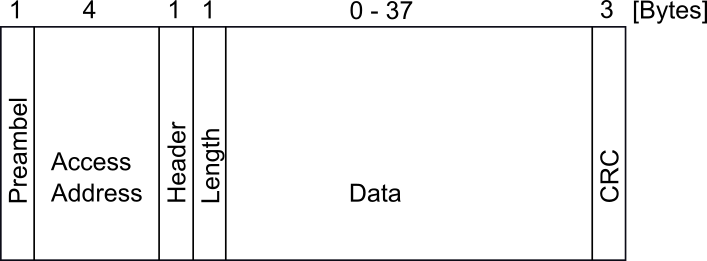
\includegraphics[width=1.0\textwidth]{2TheoretischeGrundlagen/imag/BLE_Paketstruktur.png}
    \caption{BLE Paketstruktur}
    \label{ble_paket} 
\end{figure}



